\PassOptionsToPackage{enable-debug,check-declarations}{expl3}
\RequirePackage{pdfmanagement-testphase}
\DeclareDocumentMetadata {  }
\ExplSyntaxOn
\pdfmanagement_add:nnn{Catalog}{Lang}{(enUS)}
\ExplSyntaxOff

% xmp metadata for pdf
% Originally used \usepackage[a-2a]{pdfx}
% \usepackage{hyperxmp} replaced it
% \RequirePackage{pdfmanagement-testphase} replaced it

\documentclass[11pt,
  english,
  a4paper,
]{article}
\usepackage{sa4ss}
\usepackage{amsmath,amssymb,array}
\usepackage{booktabs}

% From tagged-template.latex
\usepackage{lmodern}
\usepackage{ifxetex,ifluatex}
\ifnum 0\ifxetex 1\fi\ifluatex 1\fi=0 % if pdftex
  \usepackage[T1]{fontenc}
  \usepackage[utf8]{inputenc}
  \usepackage{textcomp} % provide euro and other symbols
\else % if luatex or xetex
  \usepackage{unicode-math}
  \defaultfontfeatures{Scale=MatchLowercase}
  \defaultfontfeatures[\rmfamily]{Ligatures=TeX,Scale=1}
\fi

% Use upquote if available, for straight quotes in verbatim environments
\IfFileExists{upquote.sty}{\usepackage{upquote}}{}
\IfFileExists{microtype.sty}{% use microtype if available
  \usepackage[]{microtype}
  \UseMicrotypeSet[protrusion]{basicmath} % disable protrusion for tt fonts
}{}
\makeatletter
\@ifundefined{KOMAClassName}{% if non-KOMA class
  \IfFileExists{parskip.sty}{%
    \usepackage{parskip}
  }{% else
    \setlength{\parindent}{0pt}
    \setlength{\parskip}{6pt plus 2pt minus 1pt}}
}{% if KOMA class
  \KOMAoptions{parskip=half}}
\makeatother
\usepackage{xcolor}
\IfFileExists{xurl.sty}{\usepackage{xurl}}{} % add URL line breaks if available
\hypersetup{
  pdftitle={Rebuilding analysis for quillback rockfish (Sebastes maliger) in U.S. waters off the coast of California based on the 2021 stock assessment},
  pdflang={en},
  hidelinks,
  pdfcreator={LaTeX via pandoc}}
\urlstyle{same} % disable monospaced font for URLs
\usepackage{longtable}
% Correct order of tables after \paragraph or \subparagraph
\usepackage{etoolbox}
\makeatletter
\patchcmd\longtable{\par}{\if@noskipsec\mbox{}\fi\par}{}{}
\makeatother
% Allow footnotes in longtable head/foot
\IfFileExists{footnotehyper.sty}{\usepackage{footnotehyper}}{\usepackage{footnote}}
\makesavenoteenv{longtable}
\usepackage{graphicx}
\makeatletter
\def\maxwidth{\ifdim\Gin@nat@width>\linewidth\linewidth\else\Gin@nat@width\fi}
\def\maxheight{\ifdim\Gin@nat@height>\textheight\textheight\else\Gin@nat@height\fi}
\makeatother
% Scale images if necessary, so that they will not overflow the page
% margins by default, and it is still possible to overwrite the defaults
% using explicit options in \includegraphics[width, height, ...]{}
\setkeys{Gin}{width=\maxwidth,height=\maxheight,keepaspectratio}
% Set default figure placement to htbp
\makeatletter
\def\fps@figure{htbp}
\makeatother
\setlength{\emergencystretch}{3em} % prevent overfull lines
\providecommand{\tightlist}{%
  \setlength{\itemsep}{0pt}\setlength{\parskip}{0pt}}
\setcounter{secnumdepth}{5}
\ifxetex
  % Load polyglossia as late as possible: uses bidi with RTL langages (e.g. Hebrew, Arabic)
  \usepackage{polyglossia}
  \setmainlanguage[]{english}
\else
  \usepackage[shorthands=off,main=english]{babel}
\fi

\providecommand{\tightlist}{%
  \setlength{\itemsep}{0pt}\setlength{\parskip}{0pt}}


\date{}
\newcommand{\trTitle}{Rebuilding analysis for quillback rockfish (\emph{Sebastes maliger}) in U.S. waters off the coast of California based on the 2021 stock assessment}
\newcommand{\trYear}{2021}
\newcommand{\trMonth}{September}
\newcommand{\trAuthsLong}{true}
\newcommand{\trAuthsBack}{Langseth, B.J., C.R. Wetzel}
\newcommand{\trCitation}{
\begin{hangparas}{1em}{1}
\trAuthsBack{}. \trYear{}. \trTitle{}. Pacific Fisheries Management Council, Portland, Oregon. \pageref{LastPage}{}\,p.
\end{hangparas}}

\AtBeginDocument{\tagstructbegin{tag=Document}}
\AtEndDocument{\tagstructend}
\pretocmd{\maketitle}{\tagstructbegin{tag=H1}\tagmcbegin{tag=H1}}{}{}
\apptocmd{\maketitle}{\tagmcend\tagstructend}{}{}

\begin{document}

%%%%% Frontmatter %%%%%

% Footnote symbols in front matter
\renewcommand*{\thefootnote}{\fnsymbol{footnote}}

\small
\thispagestyle{empty}
\pagenumbering{roman}
\noindent
\begin{center}
\title{Rebuilding analysis for quillback rockfish (\emph{Sebastes maliger}) in U.S. waters off the coast of California based on the 2021 stock assessment}
% \textnormal{\MakeTextUppercase{\trTitle{}}}
\vspace{1.5cm}
{\Large\textbf\newline{Rebuilding analysis for quillback rockfish (\emph{Sebastes maliger}) in U.S. waters off the coast of California based on the 2021 stock assessment}}
\vfill
by\\
Brian J. Langseth\textsuperscript{1}\\
Chantel R. Wetzel\textsuperscript{1}\vfill
\textsuperscript{1}Northwest Fisheries Science Center, U.S. Department of Commerce, National Oceanic and Atmospheric Administration, National Marine Fisheries Service, 2725 Montlake Boulevard East, Seattle, Washington 98112\vfill
\trMonth{} \trYear{}
\end{center}
\clearpage

% Fourth page: Colophon
\thispagestyle{empty}
\vspace*{\fill}
\begin{center}
\copyright{} Pacific Fisheries Management Council, \trYear{}\\
\end{center}
\par
\bigskip
\noindent
Correct citation for this publication:
\bigskip
\par
\trCitation{}
\clearpage

% Add TOC to pdf bookmarks (clickable pdf)
\pdfbookmark[1]{\contentsname}{toc}

% Table of contents page, lists of figures and tables
\tableofcontents\clearpage
%\listoffigures \listoftables \clearpage
\label{TRlastRoman}
\clearpage

% Table of contents
\newpage
\thispagestyle{empty} % to remove page number

% Settings for the main document
\pagenumbering{arabic}  % Regular page numbers
\pagestyle{plain}  % No page number on first page of main document, use 'empty'
\renewcommand*{\thefootnote}{\arabic{footnote}}  % Back to numeric footnotes
\setcounter{footnote}{0}  % And start at 1
\renewcommand{\headrulewidth}{0.5pt}
\renewcommand{\footrulewidth}{0.5pt}
%\pagestyle{fancy}\fancyhead[c]{Draft: Do not cite or circulate}

\newcommand{\lt}{\ensuremath <}
\newcommand{\gt}{\ensuremath >}

%Define cslreferences environment, required by pandoc 2.8
%https://github.com/rstudio/rmarkdown/issues/1649

\pagebreak
\pagenumbering{roman}
\setcounter{page}{1}

\renewcommand{\thetable}{\roman{table}}
\renewcommand{\thefigure}{\roman{figure}}

\setlength\parskip{0.5em plus 0.1em minus 0.2em}

\tagstructbegin{tag=H1}\tagmcbegin{tag=H1}

\hypertarget{summary}{%
\section*{Summary}\label{summary}}
\addcontentsline{toc}{section}{Summary}

\leavevmode\tagmcend\tagstructend

\tagstructbegin{tag=P}\tagmcbegin{tag=P}

This rebuilding analysis is for the stock of quillback rockfish (\emph{Sebastes maliger}) in waters off California. The analysis is based on the 2021 stock assessment. The 2021 assessment model estimated the quillback rockfish population to be at 14\% of the unexploited equilibrium spawning output at the beginning of 2021. This rebuilding analysis compares the results of applying a suite of potential management actions to the stock for 2023 and beyond.

\leavevmode\tagmcend\tagstructend\par

\tagstructbegin{tag=P}\tagmcbegin{tag=P}

The results of the analysis show that the value for {\tagstructbegin{tag=Formula}\tagmcbegin{tag=Formula}\(\text{T}_\text{MIN}\)\leavevmode\tagmcend\tagstructend}, the median year for rebuilding to the target level in the absence of fishing since the year of declaration (2023), is 2042. The estimated generation time for quillback rockfish was estimated to be 27 years. In conjunction with {\tagstructbegin{tag=Formula}\tagmcbegin{tag=Formula}\(\text{T}_\text{MIN}\)\leavevmode\tagmcend\tagstructend} and the mean generation time, {\tagstructbegin{tag=Formula}\tagmcbegin{tag=Formula}\(\text{T}_\text{MAX}\)\leavevmode\tagmcend\tagstructend} was estimated to be 2069. The SPR = 0.537 harvest rate generates a 50\% probability of recovery by {\tagstructbegin{tag=Formula}\tagmcbegin{tag=Formula}\(\text{T}_\text{MID}\)\leavevmode\tagmcend\tagstructend} where {\tagstructbegin{tag=Formula}\tagmcbegin{tag=Formula}\(\text{T}_\text{MID}\)\leavevmode\tagmcend\tagstructend} was set equal to 2053, an intermediate year between {\tagstructbegin{tag=Formula}\tagmcbegin{tag=Formula}\(\text{T}_\text{MIN}\)\leavevmode\tagmcend\tagstructend} and {\tagstructbegin{tag=Formula}\tagmcbegin{tag=Formula}\(\text{T}_\text{MAX}\)\leavevmode\tagmcend\tagstructend}.

\leavevmode\tagmcend\tagstructend\par

\pagebreak
\setlength{\parskip}{5mm plus1mm minus1mm}
\pagenumbering{arabic}
\setcounter{page}{1}
\renewcommand{\thefigure}{\arabic{figure}}
\renewcommand{\thetable}{\arabic{table}}
\setcounter{table}{0}
\setcounter{figure}{0}

\setlength\parskip{0.2em plus 0.1em minus 0.2em}

\tagstructbegin{tag=H1}\tagmcbegin{tag=H1}

\hypertarget{introduction}{%
\section{Introduction}\label{introduction}}

\leavevmode\tagmcend\tagstructend

\tagstructbegin{tag=H1}\tagmcbegin{tag=H1}

\hypertarget{rebuilding-calculations}{%
\section{Rebuilding calculations}\label{rebuilding-calculations}}

\leavevmode\tagmcend\tagstructend

\tagstructbegin{tag=P}\tagmcbegin{tag=P}

This rebuilding analysis was conducted using software developed by A. Punt (version 3.12h, August 2021). The steps followed were:

\leavevmode\tagmcend\tagstructend\par

\begin{itemize}
    \item Define how equilibrium spawning output ($\text{SB}_0$) will be calculated. 
    \item Define how future recruitment will be generated. 
    \item Define the fishery selectivity and allocation to be applied during rebuilding. 
    \item Decide how to include uncertainty in input parameters from the stock assessment in the rebuilding analysis. 
    \item Calculate rebuilding reference points from the most current assessment results 
    \begin{itemize}
        \item Calculate the projected year in which the stock would rebuild with a 50$\%$ probability if all future fishing mortality was eliminated ($\text{T}_\text{F}$=0).
        \item  Calculate the projected year for a 50$\%$ probability of rebuilding from the year in which the stock was first declared overfished ($\text{T}_\text{MIN}$). 
        \item Calculate the mean generation time. 
        \item Calculate the maximum allowable rebuilding time ($\text{T}_\text{MAX}$). 
    \end{itemize}
    \item Identification and analysis of alternative harvest strategies for rebuilding. 
\end{itemize}

\tagstructbegin{tag=H2}\tagmcbegin{tag=H2}

\hypertarget{definition-of-equilibrium-spawning-output}{%
\subsection{Definition of Equilibrium Spawning Output}\label{definition-of-equilibrium-spawning-output}}

\leavevmode\tagmcend\tagstructend

\tagstructbegin{tag=P}\tagmcbegin{tag=P}

The equilibrium spawning output ({\tagstructbegin{tag=Formula}\tagmcbegin{tag=Formula}\(\text{SB}_0\)\leavevmode\tagmcend\tagstructend}) used in this rebuilding analysis is calculated via the stock-recruitment relationship in order to be consistent with assessment model results. This level was estimated to be 110.16 millions of eggs in the base case assessment model, which dictates a rebuilding relative spawning output target ({\tagstructbegin{tag=Formula}\tagmcbegin{tag=Formula}\(\text{SB}_{40\%}\)\leavevmode\tagmcend\tagstructend}) of 44.07 millions of eggs (Table \ref{tab:ref-points}).

\leavevmode\tagmcend\tagstructend\par

\tagstructbegin{tag=H2}\tagmcbegin{tag=H2}

\hypertarget{generation-of-future-recruitment}{%
\subsection{Generation of future recruitment}\label{generation-of-future-recruitment}}

\leavevmode\tagmcend\tagstructend

\tagstructbegin{tag=P}\tagmcbegin{tag=P}

The estimated parameters of the stock recruitment relationship (unexploited equilibrium recruitment {[}natural log of {\tagstructbegin{tag=Formula}\tagmcbegin{tag=Formula}\(R_0\)\leavevmode\tagmcend\tagstructend}{]}, and steepness {[}{\tagstructbegin{tag=Formula}\tagmcbegin{tag=Formula}\(h\)\leavevmode\tagmcend\tagstructend}{]}) were used to generate future recruitments in the rebuilding analysis. The 2021 assessment model did not estimate annual recruitment deviations but uncertainty around future recruitments was generated by assuming a recruitment variability of {\tagstructbegin{tag=Formula}\tagmcbegin{tag=Formula}\(\sigma_R = 0.60\)\leavevmode\tagmcend\tagstructend}.

\leavevmode\tagmcend\tagstructend\par

\tagstructbegin{tag=H2}\tagmcbegin{tag=H2}

\hypertarget{fishery-selectivity-and-allocation}{%
\subsection{Fishery selectivity and allocation}\label{fishery-selectivity-and-allocation}}

\leavevmode\tagmcend\tagstructend

\tagstructbegin{tag=P}\tagmcbegin{tag=P}

The selectivity and weight-at-age used in the rebuilding analysis were obtained from 2021 assessment. The relative allocation of catch among fleets in this rebuilding analysis was informed using the relative fishing mortality averaged over recent years (2015-2019).

\leavevmode\tagmcend\tagstructend\par

\tagstructbegin{tag=H2}\tagmcbegin{tag=H2}

\hypertarget{inclusion-of-uncertainty}{%
\subsection{Inclusion of uncertainty}\label{inclusion-of-uncertainty}}

\leavevmode\tagmcend\tagstructend

\tagstructbegin{tag=P}\tagmcbegin{tag=P}

Uncertainty was included in this rebuilding analysis via 1,200 random simulations of stochastic future recruitment strengths and integration over the three states of nature across stock size, log({\tagstructbegin{tag=Formula}\tagmcbegin{tag=Formula}\(R_0\)\leavevmode\tagmcend\tagstructend}). The base model was given 50\% of the weight and each alternative state of nature was given 25\% of the weight.

\leavevmode\tagmcend\tagstructend\par

\tagstructbegin{tag=H2}\tagmcbegin{tag=H2}

\hypertarget{rebuilding-reference-points}{%
\subsection{Rebuilding reference points}\label{rebuilding-reference-points}}

\leavevmode\tagmcend\tagstructend

\tagstructbegin{tag=P}\tagmcbegin{tag=P}

Two alternative rebuilding scenarios were explored. The first set the 2021 and 2022 ACL removals at 13.4999 mt and 13.5001 mt, respectively, based on values provided by the Pacific Fishery Management Council Groundfish Management Team. The second analysis explored the impact on the rebuilding plan if removals in 2021 and 2022 were reduced to 13.5 mt for both years. The following reference points reported below are based on assumed full removals of 13.4999 and 13.5001 mt in 2021 and 2022. The reference points based on assuming lower removals in 2021 and 2022 are presented as sensitivities later in the results section.

\leavevmode\tagmcend\tagstructend\par

\tagstructbegin{tag=P}\tagmcbegin{tag=P}

All reference points calculated based on this rebuilding analysis are given in Table \ref{tab:ref-points}. The minimum time required for rebuilding, {\tagstructbegin{tag=Formula}\tagmcbegin{tag=Formula}\(\text{T}_\text{MIN}\)\leavevmode\tagmcend\tagstructend}, with no fishing (F=0) starting in 2023 was estimated to be 19 years, corresponding to the stock being rebuilt by 2042, assuming the default removals for 2021 and 2022. The mean generation time was estimated to be 27 years. The maximum time allowed for rebuilding, {\tagstructbegin{tag=Formula}\tagmcbegin{tag=Formula}\(\text{T}_\text{MAX}\)\leavevmode\tagmcend\tagstructend}, is defined as the {\tagstructbegin{tag=Formula}\tagmcbegin{tag=Formula}\(\text{T}_\text{MIN}\)\leavevmode\tagmcend\tagstructend} plus the mean generation time for stocks that require more than 10 years to rebuild. Quillback rockfish was unable to rebuild within 10 years so the estimated {\tagstructbegin{tag=Formula}\tagmcbegin{tag=Formula}\(\text{T}_\text{MAX}\)\leavevmode\tagmcend\tagstructend} was 2069.

\leavevmode\tagmcend\tagstructend\par

\tagstructbegin{tag=P}\tagmcbegin{tag=P}

{\tagstructbegin{tag=Formula}\tagmcbegin{tag=Formula}\(\text{T}_\text{TARGET}\)\leavevmode\tagmcend\tagstructend}, {\tagstructbegin{tag=Formula}\tagmcbegin{tag=Formula}\(\text{SPR}_\text{TARGET}\)\leavevmode\tagmcend\tagstructend} and {\tagstructbegin{tag=Formula}\tagmcbegin{tag=Formula}\(\text{P}_\text{MAX}\)\leavevmode\tagmcend\tagstructend} are not specified since this is the first rebuilding plan for quillback rockfish and these values have not been set via the Pacific Fishery Management Council (Council) process. A rebuilding strategy is presented below based on rebuilding target year termed {\tagstructbegin{tag=Formula}\tagmcbegin{tag=Formula}\(\text{T}_\text{MID}\)\leavevmode\tagmcend\tagstructend} which is set at 2053, mid-value between {\tagstructbegin{tag=Formula}\tagmcbegin{tag=Formula}\(\text{T}_\text{MIN}\)\leavevmode\tagmcend\tagstructend} and {\tagstructbegin{tag=Formula}\tagmcbegin{tag=Formula}\(\text{T}_\text{MAX}\)\leavevmode\tagmcend\tagstructend}, along with the associated SPR harvest rate. The Council may opt to select a {\tagstructbegin{tag=Formula}\tagmcbegin{tag=Formula}\(\text{T}_\text{TARGET}\)\leavevmode\tagmcend\tagstructend} earlier or later than this {\tagstructbegin{tag=Formula}\tagmcbegin{tag=Formula}\(\text{T}_\text{MID}\)\leavevmode\tagmcend\tagstructend} value based on fishery, economic, or other factors.

\leavevmode\tagmcend\tagstructend\par

\tagstructbegin{tag=H2}\tagmcbegin{tag=H2}

\hypertarget{alternate-rebuilding-strategies}{%
\subsection{Alternate rebuilding strategies}\label{alternate-rebuilding-strategies}}

\leavevmode\tagmcend\tagstructend

\tagstructbegin{tag=P}\tagmcbegin{tag=P}

Assuming that a constant rate of harvest will be applied throughout a rebuilding period, the basis for rebuilding alternatives can be divided into two approaches: 1) strategies based on selection of a constant harvest rate (SPR rate), or 2) strategies based selection of a {\tagstructbegin{tag=Formula}\tagmcbegin{tag=Formula}\(\text{T}_\text{TARGET}\)\leavevmode\tagmcend\tagstructend} (year for 50\% probability of recovery). This rebuilding analysis presents the following alternate strategies spread among the approaches based on the selection of a SPR harvest rate or rebuilding by a selected target year:

\leavevmode\tagmcend\tagstructend\par

\begin{itemize}
    \item Apply a range of SPR values: 0.55, 0.60, 0.65, 0.70, and 0.75 
    \item Eliminate all harvest, F = 0, beginning in the next management cycle, 2023, the same as setting a constant SPR harvest rate of 1.0.
    \item Apply the ACL based on the 40:10 harvest control rule.
    \item Apply the ABC with time-varying $\sigma$.
    \item Apply SPR harvest rates that are estimated to lead to a 50$\%$ probability of recovery by alternative target years: $\text{T}_\text{MID}$, $\text{T}_\text{MAX}$, and other years between $\text{T}_\text{MIN}$ and $\text{T}_\text{MAX}$
\end{itemize}

\tagstructbegin{tag=P}\tagmcbegin{tag=P}

All of the above rebuilding strategies were conducted assuming removals of 13.5 mt and 13.5 mt in 2021 and 2022. A sensitivity examining the impact of reducing removals in 2021 and 2022 to 50 mt was conducted on a subset of the alternative fixed SPR harvest rate alternative listed above.

\leavevmode\tagmcend\tagstructend\par

\tagstructbegin{tag=H1}\tagmcbegin{tag=H1}

\hypertarget{results}{%
\section{Results}\label{results}}

\leavevmode\tagmcend\tagstructend

\tagstructbegin{tag=P}\tagmcbegin{tag=P}

Summary results from the rebuilding alternatives assuming removals of 13.4999 and 13.5001 mt are presented in Table \ref{tab:reb-options}. Summaries of the additional alternative based on reduced removals in 2021 and 2022 are presented in Table \ref{tab:reb-options-catch} and rebuilding alternatives based on various target years are presented in Table \ref{tab:reb-options-year}.

\leavevmode\tagmcend\tagstructend\par

\tagstructbegin{tag=P}\tagmcbegin{tag=P}

The target rebuilding year based on the range of pre-specified SPR values between 0.55 - 0.75 ranged from 2036 - 2046 (Table \ref{tab:reb-options}). The probability of rebuilding by year steadily increased across the alternative SPR values with full rebuilding by 2046 when the lowest SPR of 0.55 was applied (Table \ref{tab:prob-mat} and Figure \ref{fig:prob-fig}). The recommended removals in 2023, the first year of rebuilding, were low ranging between 0.25 - 1.79 mt across alternative SPR values (Table \ref{tab:acl-mat}) with the recommended removals slowly increasing by year during the rebuilding period (Figure \ref{fig:acl-fig}). The change in spawning output by year under each of the alternative SPR values are shown by year in Table \ref{tab:ssb-mat} and Figure \ref{fig:ssb-fig}).

\leavevmode\tagmcend\tagstructend\par

\tagstructbegin{tag=P}\tagmcbegin{tag=P}

The ``ABC Rule'' projections were based on the adopted rockfish SPR target of 0.50 combined with a time-varying {\tagstructbegin{tag=Formula}\tagmcbegin{tag=Formula}\(\sigma\)\leavevmode\tagmcend\tagstructend} and category 2 {\tagstructbegin{tag=Formula}\tagmcbegin{tag=Formula}\(P^*\)\leavevmode\tagmcend\tagstructend}. The stock was estimated to rebuild by year 2053 with a probability of 0.915 (Table \ref{tab:reb-options}). Rebuilding by {\tagstructbegin{tag=Formula}\tagmcbegin{tag=Formula}\(\text{T}_\text{MID}\)\leavevmode\tagmcend\tagstructend}, 2053, was achieved using a SPR value of 0.537 (Table \ref{tab:reb-options}) with a 0.915 probability of rebuilding by {\tagstructbegin{tag=Formula}\tagmcbegin{tag=Formula}\(\text{T}_\text{MAX}\)\leavevmode\tagmcend\tagstructend}, 2069 (Table \ref{tab:prob-mat}).

\leavevmode\tagmcend\tagstructend\par

\tagstructbegin{tag=P}\tagmcbegin{tag=P}

Reducing the assumed removals in 2021 and 2022 had only a limited impact on the estimated rebuilding by SPR rate (Table \ref{tab:reb-options-catch}). Reducing the removals in 2021 and 2022 decreased the minimum time for rebuilding ({\tagstructbegin{tag=Formula}\tagmcbegin{tag=Formula}\(\text{T}_\text{MIN}\)\leavevmode\tagmcend\tagstructend}) to 2042, two years earlier compared to the initial rebuilding alternatives. The reduction of the {\tagstructbegin{tag=Formula}\tagmcbegin{tag=Formula}\(\text{T}_\text{MIN}\)\leavevmode\tagmcend\tagstructend} resulted in a decrease in the {\tagstructbegin{tag=Formula}\tagmcbegin{tag=Formula}\(\text{T}_\text{MAX}\)\leavevmode\tagmcend\tagstructend} to 2070. The probability of rebuilding, ACLs, and spawning outputs by year are shown in Tables \ref{tab:prob-mat-catch} - \ref{tab:ssb-mat-catch}.

\leavevmode\tagmcend\tagstructend\par

\tagstructbegin{tag=P}\tagmcbegin{tag=P}

The final alternative rebuilding analysis that examined a range of specific rebuilding target years (Table \ref{tab:reb-options-year}) generally fell within alternatives explored in the initial analysis (Table \ref{tab:reb-options}) but provided additional granularity to see potential rebuilding timelines. The probability of rebuilding, ACLs, and spawning output by year are shown in Tables \ref{tab:prob-mat-year} - \ref{tab:ssb-mat-year}

\leavevmode\tagmcend\tagstructend\par

\tagstructbegin{tag=H1}\tagmcbegin{tag=H1}

\hypertarget{acknowledgments}{%
\section{Acknowledgments}\label{acknowledgments}}

\leavevmode\tagmcend\tagstructend

\tagstructbegin{tag=P}\tagmcbegin{tag=P}

Here are all the mad props!

\leavevmode\tagmcend\tagstructend\par

\clearpage

\tagstructbegin{tag=H1}\tagmcbegin{tag=H1}

\hypertarget{references}{%
\section{References}\label{references}}

\leavevmode\tagmcend\tagstructend

\tagstructbegin{tag=BibEntry}\tagmcbegin{tag=BibEntry}

\hypertarget{refs}{}

\leavevmode\tagmcend\tagstructend

\clearpage

\tagstructbegin{tag=H1}\tagmcbegin{tag=H1}

\hypertarget{tables}{%
\section{Tables}\label{tables}}

\leavevmode\tagmcend\tagstructend

\clearpage

\tagstructbegin{tag=H1}\tagmcbegin{tag=H1}

\hypertarget{figures}{%
\section{Figures}\label{figures}}

\leavevmode\tagmcend\tagstructend

\tagstructbegin{tag=Figure,alttext={Summary of data sources used in the base model}}\tagmcbegin{tag=Figure}

\begin{figure}
\centering
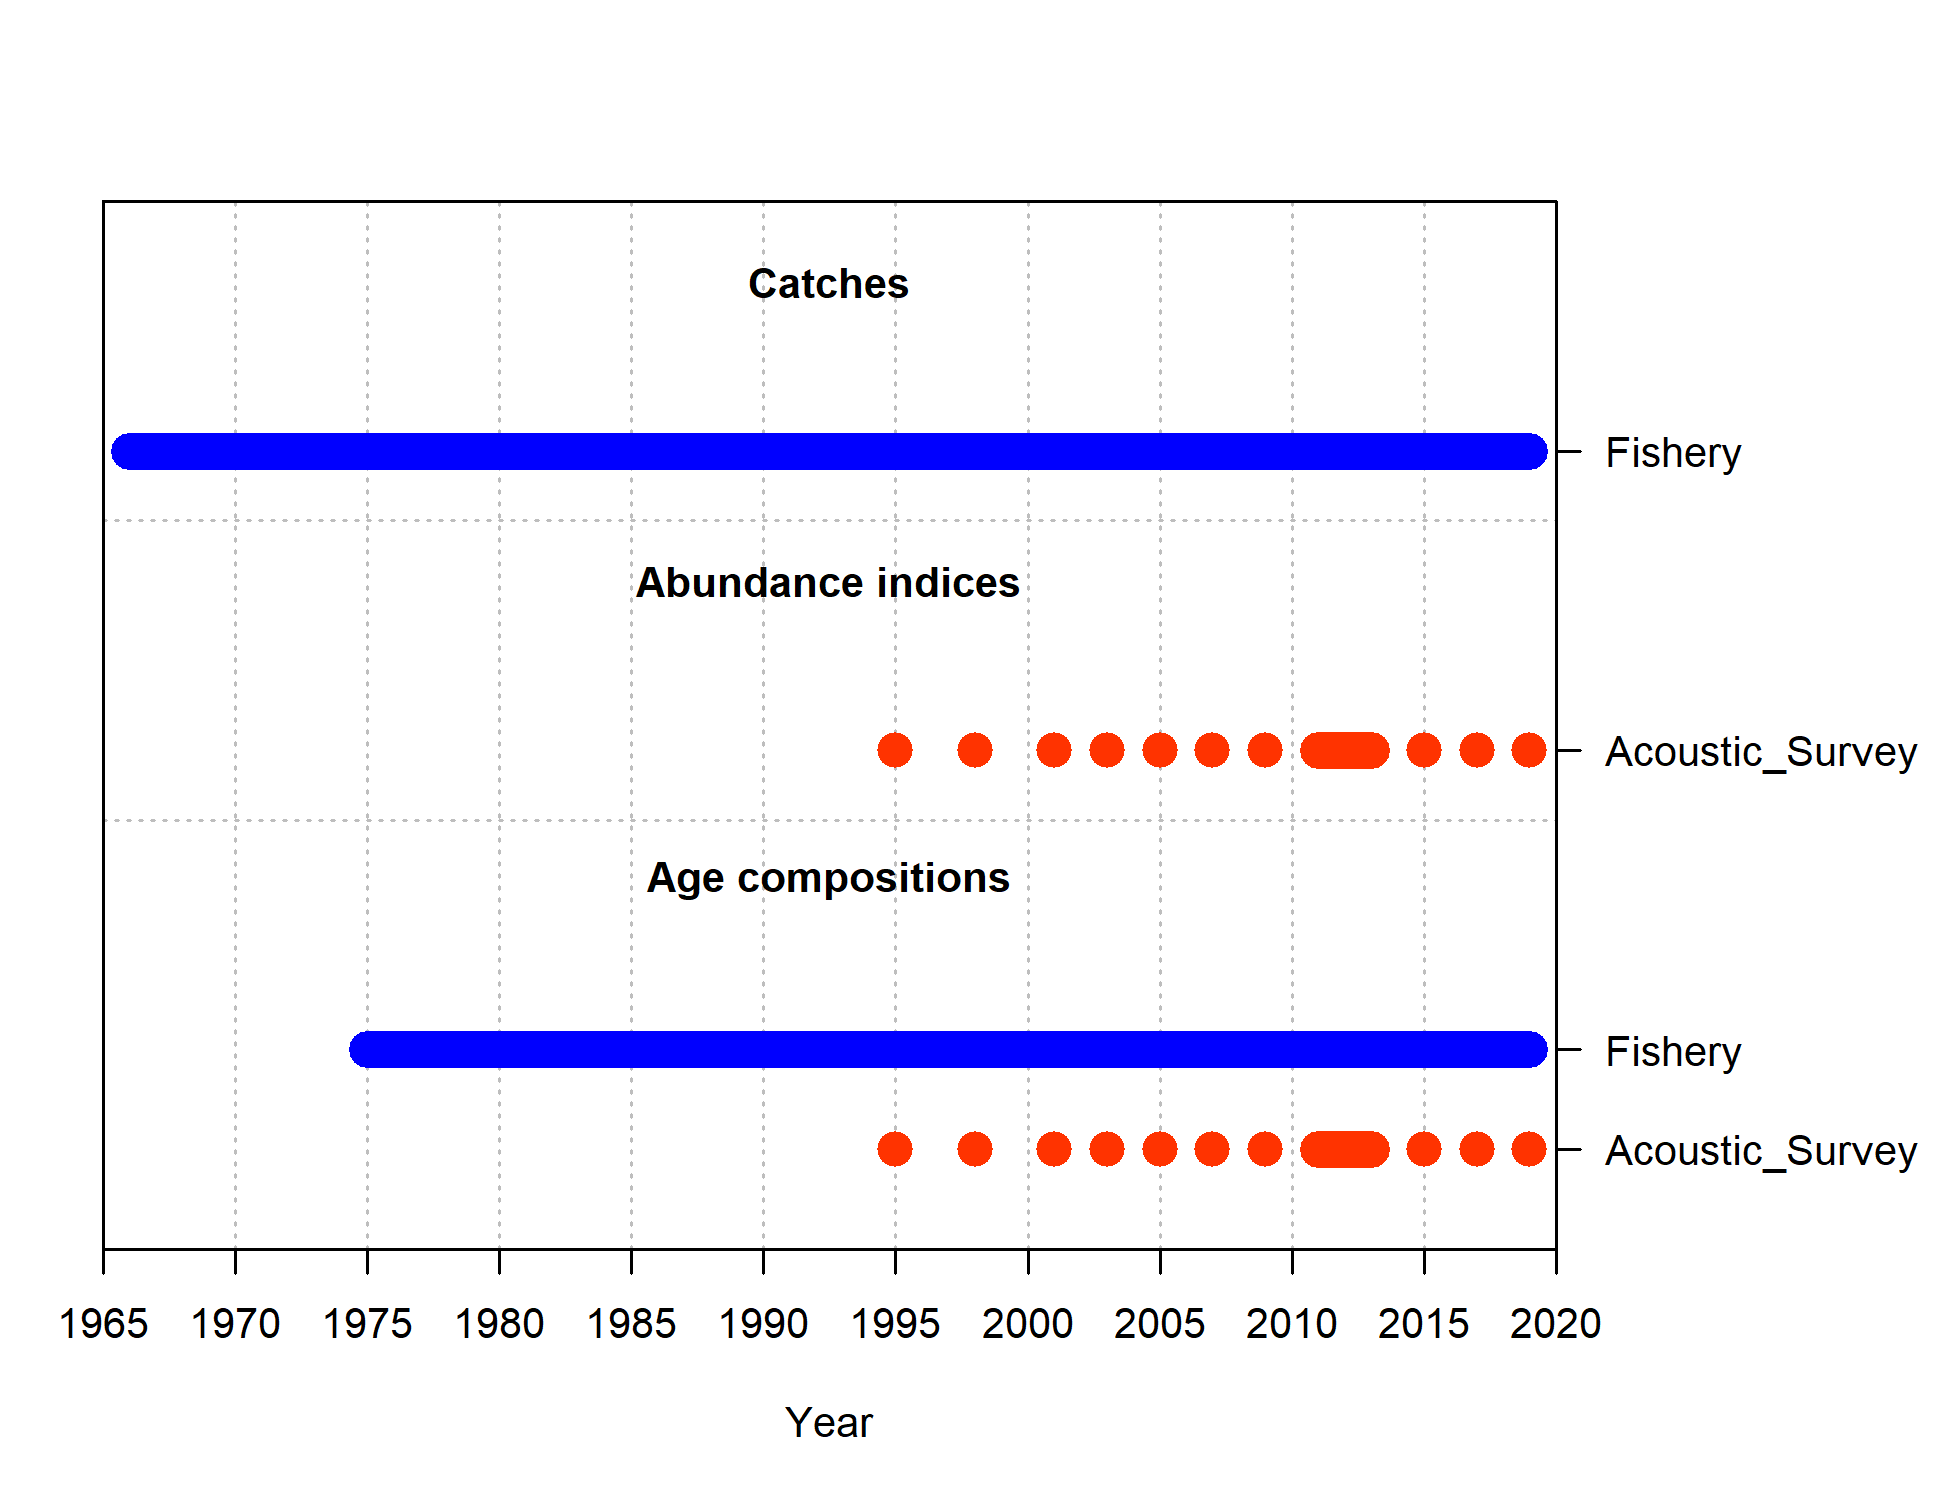
\includegraphics[width=1\textwidth,height=1\textheight]{data-plot.png}
\caption{Summary of data sources used in the base model.\label{fig:data-plot}}
\end{figure}

\tagmcend\tagstructend
\end{document}
